% !TeX program = xelatex
% !TeX encoding = utf-8
% 《机器人》LaTeX模板
% 面向往复夹持递送的血管介入机器人力反馈扰动建模与残差抑制

\documentclass{JQRnew}


% 修订标记：正文及公式按原稿逐段对照；干净版关闭颜色。
\providecommand{\RevisionColor}{\color{black}}
\newcommand{\revised}[1]{{\RevisionColor#1}}
\newcommand{\revbegin}{\begingroup\RevisionColor}
\newcommand{\revend}{\par\endgroup}

\JQRsetup{
 % 期刊出版信息
 volume     = xx,
 number     = x,
 year       = 2026,
 month      = 10,
 doi        = 240001,
 % 通信作者
 corrauthor = {\revised{胡琨元（Email待补）；刘浩，Email: liuhao@sia.cn}},
 % 日期
 dates      = {2026-10-21/2026-10-21/2026-10-21},
 %
 % ---- 中文相关信息
 cntitle    = {面向往复夹持递送的血管介入机器人力反馈扰动建模与残差抑制},
 cnauthor   = {隋凯丞\addr{1,2,3}, 郑力铭\addr{1,2,3}, 林\quad 鹏\addr{1,2}, 胡琨元\addr{1,2*}, 刘\quad 浩\addr{1,2*}},
 runtitle   = {隋凯丞，等：面向往复夹持递送的血管介入机器人力反馈扰动建模与残差抑制},
 cnaddress  = {1. 中国科学院沈阳自动化研究所 机器人学国家重点实验室，辽宁~~沈阳\quad 110016；\\
               2. 辽宁省微创手术机器人重点实验室，辽宁~~沈阳\quad 110016；\\
               3. 中国科学院大学，北京\quad 100049},
 %
 % ----- 中文摘要
 cnabstract = {\replaced{夹持式血管介入机器人能够直接测量器械近端力，但有限的导轨行程使其在输送中必须反复回退和重新夹持，这一过程中，长距离输送需要较大空间且有屈曲风险，重新夹持则会造成操作中断和力觉波动。因此，需要研究有限行程约束下兼顾输送连续性、运动精度与力觉稳定性的控制方法，以提高机器人辅助介入的可靠性和安全性。}{【目的】为了将夹持式血管介入机器人往复运动中周期性扰动的力反馈，建立轴向力反馈重构方法。}【方法】根据动作特征将递送与交接过程划分，建模测量信号中的惯性与零载，利用递送稳态载荷和S8末实测承载确定轴向补偿初值。以前向推进行程建立包含弹性恢复与附加阻力衰减的双指数恢复模型；将换手后的恢复行程划分为20个单元，以门控循环单元（GRU）逐单元编码，再对此前最多10个周期同一单元的编码进行注意力加权，在不输入实时测力的条件下估计轴向残差。S2～S8保持锁存值，S9对残差限幅并淡入，在恢复完成、停止或回拉时撤除补偿。扭矩通道仅进行测量校正与交接锁存。参考载荷由往复递送数据去除交接段后按插入深度拼接得到，并用分段恒速连续递送数据检验。【结果】评价轴向反馈误差、全周期波动及阻力阶跃响应，并进行消融、网络结构对比和血管模型操作者实验。重构误差、阶跃保留比、介入总时间与成功率结果为[待补]。【结论】所建方法将轴向实测载荷与恢复补偿分别处理，用于往复夹持递送中的轴向力反馈重构。},
 % ---- 中文关键字
 cnkeywords = {\revised{介入机器人；往复夹持；轴向力反馈；载荷恢复；门控循环单元；跨周期注意力}},
 %
 % ---- 英文相关信息
 entitle    = {Disturbance Modeling and Residual Suppression of Force Feedback for Vascular Intervention Robot in Reciprocating Clamping Delivery},
 enauthor   = {\revised{SUI Kaicheng\addr{1,2,3}, ZHENG Liming\addr{1,2,3}, LIN Peng\addr{1,2}, HU Kunyuan\addr{1,2*}, LIU Hao\addr{1,2*}}},
 enaddress  = {1. \textit{State Key Laboratory of Robotics, Shenyang Institute of Automation, Chinese Academy of Sciences, Shenyang} 110016, \textit{China}; \\
               2. \textit{Key Laboratory of Minimally Invasive Surgical Robot, Liaoning Province, Shenyang} 110016, \textit{China}; \\
               3. \textit{University of Chinese Academy of Sciences, Beijing} 100049, \textit{China}},
 %
 % ---- 英文摘要
 enabstract = {[Objective] An axial force feedback reconstruction method is developed for measurement fluctuations during reciprocating clamping delivery. [Methods] The delivery and handover cycle is divided into stages S1--S10. Inertia and the zero-load baseline are corrected, and the initial axial compensation is determined from the stored load at the end of S1 and the measured load at the end of S8. A double-exponential model describes elastic recovery and decay of an additional resistance term as functions of forward travel. The recovery travel after handover is divided into 20 units; a gated recurrent unit (GRU) encodes the units in order, and attention over the same unit in up to 10 preceding cycles aggregates the encodings to estimate the axial residual without real-time force inputs. The feedback is held during S2--S8; in S9 the residual is limited and introduced gradually, and compensation is withdrawn upon recovery completion, stopping, or retraction. Torque feedback uses measurement correction and holding during handover. The reference load is constructed from reciprocating delivery data by removing the handover segments and joining the remaining data by insertion depth, and it is checked against segmented constant-speed continuous delivery. [Results] Axial feedback errors, cycle-level fluctuations, and resistance-step responses are evaluated, together with ablation tests, network structure comparisons, and operator tasks in a vascular phantom. Reconstruction errors, step retention ratios, intervention times, and success rates are [to be added]. [Conclusions] The method handles the measured axial load and the recovery compensation separately for axial force feedback in reciprocating clamping delivery.},
 %
 % ---- 英文关键字
 enkeywords = {\revised{intervention robot; reciprocating clamping; axial force feedback; load recovery; gated recurrent unit (GRU); cross-cycle attention}}
}

% ----- 加载宏包
\usepackage{algorithm}
\usepackage{algpseudocode}
\usepackage{pifont}
\usepackage{balance}
\usepackage{mwe}
\usepackage{booktabs}
\usepackage{amsmath,amssymb}
\usepackage{bm}
\usepackage{enumitem}
\usepackage{float}
\usepackage[draft,commentmarkup=footnote]{changes}
\usepackage{xeCJKfntef}
\setdeletedmarkup{\CJKsout{#1}}

\floatname{algorithm}{算法}
\renewcommand{\algorithmicrequire}{\textbf{输入:}}
\renewcommand{\algorithmicensure}{\textbf{输出:}}
\newcommand{\algorithmicchushi}{\textbf{初始化:}}

\begin{document}

\maketitle

% 引言部分不设节标题（遵循《机器人》期刊约定）
血管介入机器人通过主从遥操作驱动导丝和导管完成推进与旋转，使术者能够免遭X射线辐射伤害\ucite{ref2}。在手动递送中，术者通过指端感受器械阻力，并结合影像判断器械的运动与受力状态，但在遥操作中，这种触觉联系需要通过从端测量和主端力反馈重建。手术机器人力反馈相关研究指出，从端接触力的测量、主端力的再现以及反馈控制的稳定性\comment{这里好像根本没有提到力反馈干扰会打破反馈控制的稳定性}共同影响术者获得的触觉信息\ucite{ref29}，力反馈既需要反映器械与环境之间的相互作用，也需要减少不必要的干扰波动，使术者能够辨别操作阻力的变化。

从测量位置看，血管介入机器人相关的力感知可分为体内远端测力和体外近端测力。远端方案将微型传感元件集成于器械尖端以获取局部接触力，例如He等\ucite{ref3}在导管尖端集成光纤布拉格光栅传感器，测量导管与血管壁的接触力，这类方案需要兼顾器械尺寸、传感元件封装和弯曲性能，且在手术器械上集成传感器，会带来成本、组织兼容性等问题。
% 在首页自然进入第二栏的位置为模板页脚预留空间。
\JQRpubidadjcol
近端方案则在体外驱动机构的传力路径中布置力传感器\ucite{ref6,ref8}，或利用驱动电机电流估计载荷\ucite{ref5}。这类方法可与常规器械配合使用，获取沿器械传递的综合操作阻力，其中既包含尖端接触作用，也包含器械与鞘管、管腔之间的摩擦作用\ucite{ref2,ref7}。由于驱动与测力共用器械接触和传力部件，机构摩擦、惯性及姿态变化也会影响测量结果。针对这一问题，Duan等\ucite{ref17}采用杠杆放大式测力结构，缩短传力路径并减小摩擦与惯性对测量的影响。因此，近端测力的准确性不仅取决于传感器性能，还与器械驱动方式及其传力过程有关\comment{这段逻辑不对，叙述太乱。第一句不变，然后在“由于驱动与...”前方加一段，表示的大意是近端测力效果同时受近端夹持器械的机构构型影响，然后阐述目前夹持机构可以分成仿人类手指的平面夹持，一类是滚轮式的机构，然后阐述滚轮式的相关研究有什么，总结时说滚轮式的首先所需夹持力可能较大，可能使器械变形或破坏涂层。然后开始介绍夹持式的机构，这种通过机构在滑轨（或者齿轮齿条，或者丝杠，总之是这类零件，要总结一个合理的名词，是常见且符合这里意思的，不要生搬硬套）上平移，并设置内部机构旋转，使平移和旋转解耦，测量效果更好，然而夹持式有限的导轨行程使其在输送中必须进行往复运动，过程中伴随着对器械的反复重新夹持，这带来了受力状态的改变及力反馈扰动，也极大干扰了术者的感知}。

滚轮驱动通过滚轮与器械之间的摩擦实现连续输送，夹持驱动则通过夹爪夹紧器械并带动其平移\ucite{ref5,ref7}。受单次平移行程限制，往复夹持机构需要在递送与回程之间完成载荷交接。以移动夹持器递送、固定夹持器保持器械的结构，通过两者交替夹持将有限行程转换为长距离递送\ucite{ref2,ref3}；Cao等\ucite{ref10}进一步通过往复递送和多操作器协同实现多器械操作。另一类结构采用双移动夹持器，Al-Ahmad等\ucite{ref7}通过编织套筒夹持器的速度匹配与重叠夹持维持器械连续运动。这些方案在回程期间的器械运动和承载方式上存在差别。对于传感器安装于移动主爪、由固定夹持器接替承载的结构，移动主爪释放后，其测力支路随之卸载；空载回程的加减速与夹爪开闭又会引入附加瞬态载荷。重新推进时，停止后的器械载荷还需要随运动重新建立，使换手期的力反馈同时受到机构运动与承载状态变化的影响。

针对机构运动引入的附加分量，现有研究通过运行偏置标定与动力学分析建立补偿关系。Sankaran等\ucite{ref5}利用空载运行电流及其与转速的关系标定近端力估计偏置；Bao等\ucite{ref8}综合考虑摩擦、重力和旋转速度，建立与载荷及转速相关的补偿模型；Wang等\ucite{ref12}分析递送机构的平移和旋转动力学，并通过夹紧与松开器械的对比试验评价测力误差。这些方法着重分离机构运行对近端测量的影响，而主爪脱离器械时，测力支路已不再传递器械外载，单纯扣除运行偏置不能恢复该阶段的载荷信息。保持换手前的反馈值可以避免卸载跳变直接传至主端，但若在重新推进起点立即切回实测信号，停止前后的载荷差异会重新出现在反馈中；若将保持延长至载荷恢复结束，又会推迟新增阻力的反馈。因此，交接期的输出连续性需要与恢复推进后的实时受力响应共同考虑。

重新推进时的载荷变化与传力部件的变形及接触界面的摩擦状态有关。弹性夹持垫和测力元件在卸载、静止与重新承载过程中经历变形调整，黏弹性接触研究揭示了加载历史对接触载荷和接触区域演化的影响\ucite{ref20}。器械重新推进还改变其与鞘管、管腔之间的摩擦接触状态；动态摩擦模型表明，预滑移、起动摩擦和黏滑转换使摩擦力具有运动历史依赖性\ucite{ref28}。在柔性腱鞘传动中，Sun等\ucite{ref30}通过分布式摩擦与弹性伸长建模表明，局部曲率及其沿路径的位置会改变张力分布和总伸长量，说明接触路径也是影响柔性传力变形的重要因素。对于往复递送，接触变形的重新加载与起动附加阻力的演化共同影响近端载荷恢复，因而需要描述停止前后载荷之间的过渡过程。低阶模型能够以少量参数描述这一过程的主要趋势，但随着器械插入位置和接触分布改变，固定参数模型仍会产生与递送状态和运动历史有关的预测偏差。

时序学习为描述历史相关的受力关系提供了方法。Lyu等\ucite{ref13}将软体夹持器的视觉形变、夹持间距和运动速度序列输入长短期记忆网络（LSTM），估计器械操作力与扭矩；Wang等\ucite{ref14}采用时间卷积网络（TCN）学习近端测量与远端接触力之间的映射。这些方法利用历史信息估计操作载荷或远端接触力，而换手后的反馈恢复还涉及交接前后承载状态的衔接。对于解析模型难以描述的偏差，物理模型与学习方法的结合可通过残差补偿或力学约束实现。在机械臂接触力估计中，卷积神经网络被用于补偿动力学观测器的估计误差\ucite{ref21}，时序残差学习进一步将关节动力学偏差与末端力估计偏差分级修正\ucite{ref22}；柔性手术机器人研究则将准静态力学关系引入LSTM，以约束形状与接触力的预测\ucite{ref27}。上述研究将物理关系用于载荷估计，并通过数据拟合补充实际受力过程的描述。对于往复夹持递送，尚需区分载荷恢复偏差与新增外部阻力：二者可能在重新推进时同时出现，仅依据波形平滑程度或变化快慢难以分离。当实时测力值参与补偿量预测时，新增阻力也会进入补偿计算，其在反馈中的保留程度取决于训练目标、网络输入以及补偿量与实测值的组合方式。因此，恢复过程的建模与残差修正需要同时考虑对真实阻力变化的响应。

针对上述问题，有必要研究往复夹持递送中的力反馈波动抑制方法，在改善反馈连续性的同时保留真实阻力变化。

\section{问题描述（Problem description）}

\subsection{往复夹持递送过程}

\revbegin
本文研究的夹持式血管介入机器人采用主、副双夹爪交替夹持器械，通过夹爪与器械表面的摩擦接触传递运动和载荷。主夹爪安装于沿直线导轨移动的滑台上，负责器械的轴向推进与周向旋转，其内部集成轴向与周向两路测力支路；副夹爪安装于近血管鞘入口端，在主夹爪释放与回退期间保持器械位置。
\revend

\revbegin
受直线导轨行程限制，长距离递送由周期性短行程往复运动完成。根据运动和夹持时序，将一个往复周期划分为S1～S10十个阶段，如图\ref{fig1}所示。
\begin{enumerate}[label=\arabic*),nosep,itemsep=0pt,topsep=2pt,partopsep=0pt,parsep=0pt,leftmargin=2\ccwd]
\item 递送与停止（S1～S2）：主爪独立夹持器械推进，并可同时旋转（S1）；单次行程结束时滑台减速停止，副爪尚未闭合（S2）。
\item 卸载交接（S3～S4）：副爪闭合，两爪共同夹持器械（S3）；随后主爪释放，由副爪承载（S4）。
\item 空载回程（S5～S6）：主爪脱离器械后沿导轨退回（S5），在起点减速停止（S6），期间器械由副爪保持。
\item 重新承载与递送（S7～S10）：主爪在起点闭合，两爪再次共同夹持（S7）；副爪释放后，静止的主爪独立承载（S8）；主爪恢复前向推进，轴向载荷逐步恢复（S9）；恢复完成后进入稳定承载阶段（S10）。
\end{enumerate}
\revend

\revbegin
\begin{figure}[H]
\RevisionColor
\centering
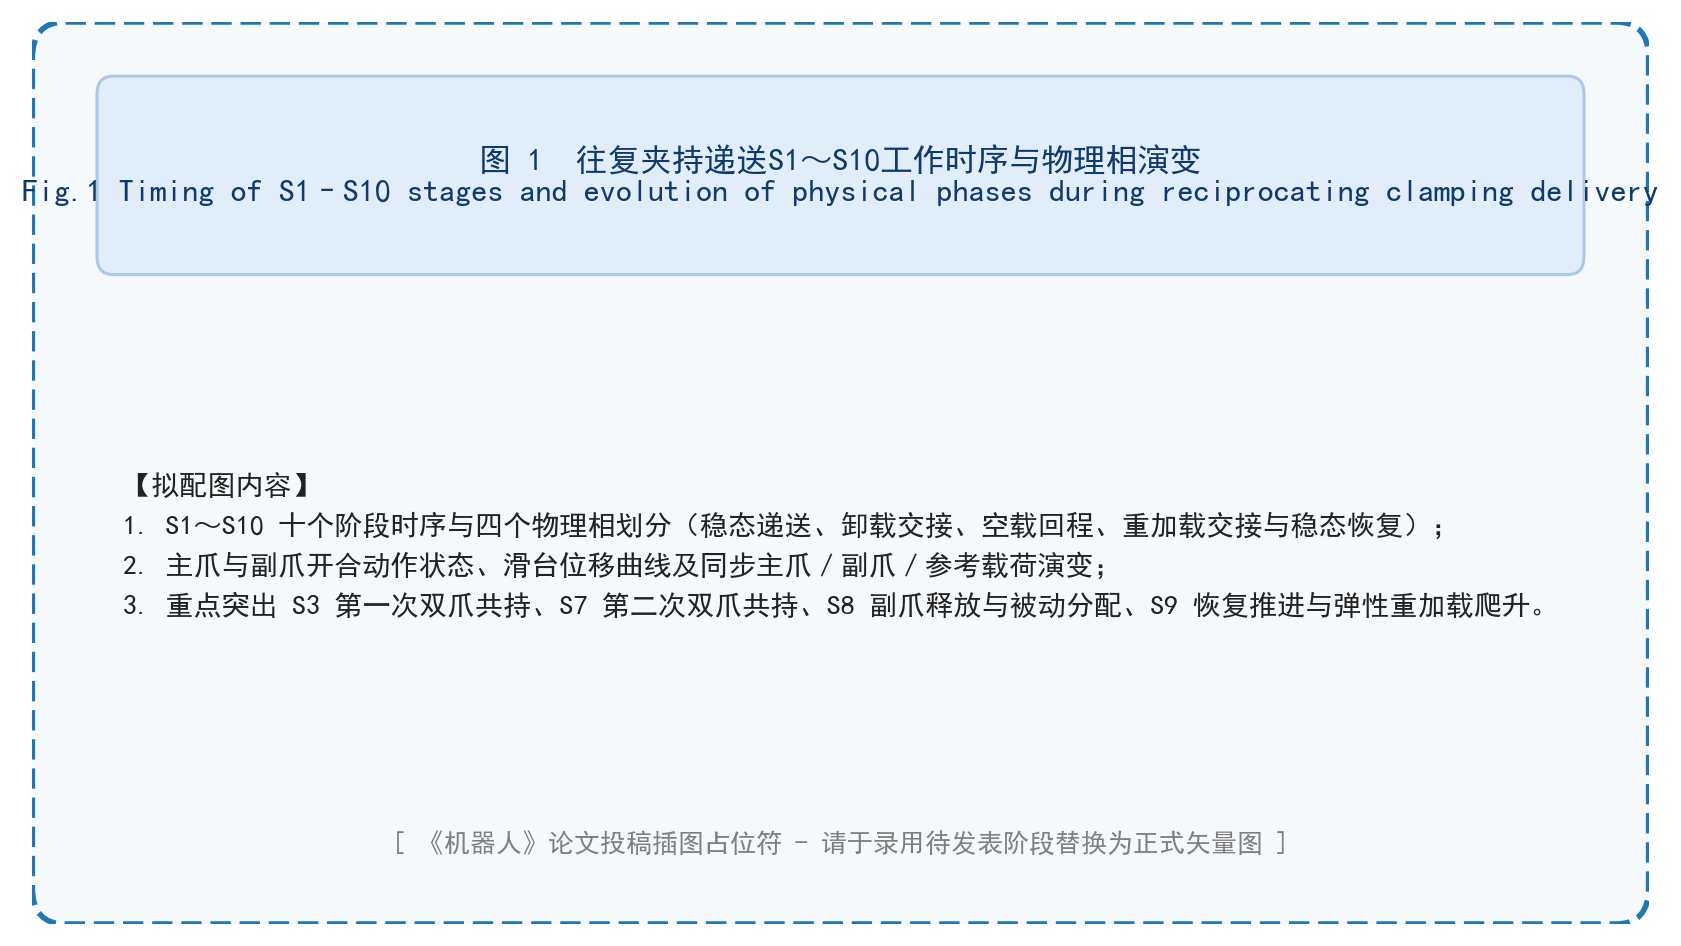
\includegraphics[width=\linewidth]{fig1.png}
\bicaption{\revised{往复夹持递送工作过程}}{\revised{Stages of reciprocating clamping delivery}}
\label{fig1}
\end{figure}
\revend

\subsection{测力波动与补偿目标}

\revbegin
往复递送过程中，主爪测力支路经历承载、卸载和重新承载。滑台启停产生轴向惯性力，旋转加减速产生附加力矩，旋转姿态还会改变零载基线。夹爪开合冲击、停止后的载荷松弛及重新推进时的载荷恢复，使近端测量信号出现周期性波动。
\revend

本文以不换手连续递送时的器械载荷作为反馈目标，参考载荷由往复递送数据构造（2.1节）。在S1末锁存稳态载荷，S2～S8保持该值；S9以前向推进行程描述轴向载荷恢复，并由两级残差网络修正恢复模型的残差；轴向输出由校正测量值与补偿量相加得到。扭矩通道只进行测量校正和S2～S8锁存，S9起输出校正测量值。

\revbegin
全文设轴向正方向沿器械名义中心轴指向远端，旋转角正方向遵循右手定则。力、扭矩、位移、角位移和时间的单位分别为 $\mathrm{N}$、$\mathrm{N}\cdot\mathrm{mm}$、$\mathrm{mm}$、$\mathrm{rad}$ 和 $\mathrm{s}$。轴向传感器读数记为 $F_{xm}$，周向支路的切向力读数记为 $F_{tm}$，经标定等效力臂 $\ell_s$ 换算得到测量扭矩 $\tau_{xm}=\ell_sF_{tm}$。输出至主端的反馈信号统一记为 $\bm w_{\mathrm{fb}}=[F_{\mathrm{fb}},\tau_{\mathrm{fb}}]^{\rm T}$。
\revend

\subsection{本文工作}

本文围绕往复夹持递送中的轴向力反馈重构开展以下工作。
\begin{enumerate}[label=\arabic*),nosep,itemsep=0pt,topsep=2pt,partopsep=0pt,parsep=0pt,leftmargin=2\ccwd]
\item 建立测量干扰模型和双爪交接受力关系，以S1末稳态载荷和S8末实测载荷确定轴向重加载补偿的初值。
\item 建立以前向推进行程为自变量的轴向载荷恢复模型，结合两级残差网络修正、交接锁存和补偿量平滑撤除，形成分阶段反馈方法。
\item 通过参数辨识、参考误差、阻力突变及消融实验评价轴向力重构，并在血管模型中比较操作时间和通过成功率；扭矩通道评价测量校正与锁存效果。
\end{enumerate}

\revbegin
第2节介绍受力关系、轴向载荷恢复模型与反馈方法，第3节给出实验配置和评价方法，第4节与第5节分别为讨论和结论。
\revend

\section{往复夹持传力与反馈补偿方法（Load transmission and feedback compensation for reciprocating clamping）}

\subsection{测量关系、双爪交接受力与参考载荷}

主爪测力支路与双爪交接关系如图\ref{fig2}所示。主、副爪之间的器械段不与其他物体接触，副爪远端的管壁接触及实验加载装置对器械的作用均计入外载。忽略器械自身惯性，轴向力和绕轴扭矩满足
\begin{equation}
\label{eq:balance}
\begin{cases}
F_M+F_S=F_{\mathrm{out}},\\
\tau_M+\tau_S=\tau_{\mathrm{out}}.
\end{cases}
\end{equation}
式中，$F_M,\tau_M$ 与 $F_S,\tau_S$ 分别为主、副爪作用于器械的轴向推力和驱动扭矩，以向远端推进和按右手定则正转为正；$F_{\mathrm{out}},\tau_{\mathrm{out}}$ 为外部轴向合阻力和合阻力矩，以阻碍上述正向运动为正。记 $\bm w_M=[F_M,\tau_M]^{\rm T}$。副爪完全释放时 $F_S=\tau_S=0$，外载全部由主爪平衡。

将轴向力与换算后的扭矩组成测量向量 $\bm y=[F_{xm},\ell_sF_{tm}]^{\rm T}$。传感器连接浮动传力组件与滑台，浮动组件的轴向弹性位移较小，其加速度近似取滑台加速度。测量关系写为
\begin{align}
\label{eq:measurement}
\bm y={}&\bm H_0\bm w_M+\bm p_{\mathrm{iner}}(\bm q_M)
+\bm b(\varphi_M)\notag\\
&+\bm p_{\mathrm{clamp}}(t)+\bm\varepsilon,\\
\label{eq:inertia}
\bm p_{\mathrm{iner}}(\bm q_M)={}&
\begin{bmatrix}m_sa_M\\J_s\alpha_M\end{bmatrix}.
\end{align}
式中，$\bm q_M=[x_M,\dot x_M,a_M,\varphi_M,\dot\varphi_M,\alpha_M]^{\rm T}$ 为平移轴和旋转轴的位置、速度及加速度；$m_s$ 和 $J_s$ 为两支路的等效质量和转动惯量，单位与毫米制运动量相匹配；$\bm H_0\in\mathbb R^{2\times2}$ 为离线标定的可逆传递矩阵，非对角元包含力与扭矩之间的单位换算；$\bm b(\varphi_M)$ 为零载基线，包含静态零偏和随旋转角变化的重力分量；$\bm\varepsilon$ 为测量噪声。各向量的两个分量依次以 $\mathrm{N}$ 和 $\mathrm{N}\cdot\mathrm{mm}$ 计。

开合指令记为 $\bm c=[c_M,c_S]^{\rm T}\in\{0,1\}^2$，闭合取1、释放取0。$\bm p_{\mathrm{clamp}}(t)$ 为夹爪开合引起的短时冲击。开合动作发生在S3、S4、S7和S8，这些阶段的反馈采用锁存值，因此不对 $\bm p_{\mathrm{clamp}}$ 作在线补偿。扣除惯性项与零载基线后的校正测量值为
\begin{equation}
\label{eq:corrected-measurement}
\bm w_{\mathrm{meas}}[k]=\bm H_0^{-1}\!\left[
\bm y[k]-\bm p_{\mathrm{iner}}(\bm q_M[k])-\bm b(\varphi_M[k])\right].
\end{equation}

单爪递送阶段（S1、S9、S10）副爪完全释放，主爪独自平衡外载。S3～S7中副爪参与或独自承载（$F_S\neq0$），主爪测力支路在S4～S6卸载，并在S7原位重新闭合。由于夹持垫与传力支路存在柔顺性，S7主爪刚闭合时尚未形成明显的切向变形，外载仍主要由副爪承担，此时主爪读数不反映外载。S8副爪释放后，静止的主爪重新独自承载；交接过程中支路的部分变形已经释放，S8末主爪实测载荷低于换手前的稳态值。取S8末副爪释放冲击衰减后、平移轴与旋转轴均静止（$a_M=\alpha_M=0$）的采样时刻 $k_9$，主爪承载的初值为
\begin{equation}
\label{eq:initial-load}
\widehat{\bm w}_{M,k_9}
=\bm H_0^{-1}\!\left[\bm y[k_9]-\bm b(\varphi_M[k_9])\right].
\end{equation}

反馈的目标是不换手连续递送时的器械载荷。以累计有效插入深度 $s$ 为自变量（空载回程不计入），参考载荷记为 $\bm w_{\mathrm{ref}}(s)=[F_{\mathrm{ref}}(s),\tau_{\mathrm{ref}}(s)]^{\rm T}$。同一次递送无法同时得到换手与不换手两种载荷，因此本文由往复递送数据构造参考载荷：S1与S10取校正测量值 $\bm w_{\mathrm{meas}}$，按插入深度拼接；S2～S8期间插入深度不变，参考值取该深度处的值；S9区间以S1末段和S10初段的校正测量值按插入深度作线性最小二乘拟合，
\begin{equation}
\label{eq:reference}
\bm w_{\mathrm{ref}}(s)=\bm a_0+\bm a_1s,\quad s\in[s_9,s_{10}],
\end{equation}
式中，$s_9$ 和 $s_{10}$ 分别为S9起点和S10起点的插入深度，S10起点按实测轴向载荷进入稳态误差带的位置离线确定；$\bm a_0,\bm a_1$ 为拟合系数。该构造基于以下假设：不换手时，器械载荷在数毫米的恢复行程内随插入深度平缓变化。这一假设用分段恒速连续递送数据检验（3.2节）。

\begin{figure}[H]
\centering
\fbox{\parbox{0.92\linewidth}{\raggedright [图2待补：主爪轴向和切向测力支路、传感器力臂 $\ell_s$、惯性项及零载基线；S7与S8主副爪受力图，标出 $F_M,F_S,F_{\mathrm{out}}$。S8副爪完全释放，主爪独立承载。]}}
\bicaption{测力支路与双爪交接受力关系}{Force-sensing branches and load transfer during gripper handover}
\label{fig2}
\end{figure}

\subsection{换手后重新推进阶段的轴向载荷恢复模型}

在S1匀速段末锁存连续递送的局部参考值
\begin{equation}
\label{eq:lock}
\widehat{\bm D}_9=\frac{1}{N_{\mathrm{lock}}}
\sum_{j=k_{\mathrm{S1,end}}-N_{\mathrm{lock}}+1}^{k_{\mathrm{S1,end}}}
\bm w_{\mathrm{meas}}[j].
\end{equation}
式中，$k_{\mathrm{S1,end}}$ 为减速指令发出前的最后一个采样时刻，$N_{\mathrm{lock}}$ 为完全位于匀速段内的窗口长度。轴向初始载荷缺口为
\begin{equation}
\label{eq:deficit}
\widehat A_{9,F}=\widehat D_{9,F}-\widehat w_{M,k_9,F}.
\end{equation}

恢复模型用于 $\widehat A_{9,F}>0$ 的前向推进过程。自S8末起累计前向推进行程
\begin{equation}
\label{eq:recovery-travel}
s_{\mathrm{rec}}(t)=\int_{t_{\mathrm{S8,end}}}^{t}
\max\!\left(\dot x_M(t'),0\right)\,\mathrm dt'.
\end{equation}
本文假设恢复初期的载荷增长主要来自传力链的弹性恢复，停顿后的附加摩擦阻力随推进行程衰减。令 $w_F(s_{\mathrm{rec}})$ 为模型给出的轴向载荷，采用一阶恢复关系
\begin{equation}
\label{eq:recovery-ode}
\frac{\mathrm dw_F}{\mathrm ds_{\mathrm{rec}}}
=\frac{\widehat D_{9,F}+\Delta_F e^{-s_{\mathrm{rec}}/D_c}-w_F}{\lambda_F}.
\end{equation}
式中，$\lambda_F>0$ 为弹性恢复的特征行程，$\Delta_F\ge0$ 为停顿后附加阻力的幅值，$D_c>0$ 为附加阻力衰减的特征行程。三个参数在各推进速度下取同一组数值。以 $w_F(0)=\widehat w_{M,k_9,F}$ 为初值积分，得到相对于锁存参考值的补偿量
\begin{equation}
\label{eq:recovery-comp}
\begin{aligned}
f_{\mathrm{rel},F}(s_{\mathrm{rec}})&=\widehat D_{9,F}-w_F(s_{\mathrm{rec}})\\
&=\widehat A_{9,F}e^{-s_{\mathrm{rec}}/\lambda_F}\\
&\quad-\frac{\Delta_FD_c}{D_c-\lambda_F}
\left(e^{-s_{\mathrm{rec}}/D_c}-e^{-s_{\mathrm{rec}}/\lambda_F}\right).
\end{aligned}
\end{equation}
当 $D_c=\lambda_F$ 时，取极限形式
\begin{equation}
\label{eq:equal-scales}
f_{\mathrm{rel},F}(s_{\mathrm{rec}})=
\left(\widehat A_{9,F}-\Delta_F\frac{s_{\mathrm{rec}}}{\lambda_F}\right)e^{-s_{\mathrm{rec}}/\lambda_F}.
\end{equation}
当 $\Delta_F=0$ 时，式\eqref{eq:recovery-comp}退化为单指数恢复。若恢复曲线出现高于锁存参考值的峰值，$f_{\mathrm{rel},F}$ 在峰值附近为负，即从实测值中扣除附加阻力分量。

恢复起点的加载斜率为
\begin{equation}
\label{eq:initial-slope}
\begin{aligned}
k_0&=\left.\frac{\mathrm dw_F}{\mathrm ds_{\mathrm{rec}}}\right|_{s_{\mathrm{rec}}=0}
=\frac{\widehat A_{9,F}+\Delta_F}{\lambda_F},\\
\lambda_F&=\frac{\widehat A_{9,F}+\Delta_F}{k_0}.
\end{aligned}
\end{equation}
按该模型，在初始加载斜率相近的条件下，待恢复载荷 $\widehat A_{9,F}+\Delta_F$ 越大，恢复所需行程越长。逐周期拟合得到的 $\lambda_F$ 与 $k_0$ 用于检查这一关系（3.2节）。

令式\eqref{eq:recovery-ode}右端为零，得到峰值对应的行程
\begin{equation}
\label{eq:peak-location}
\begin{aligned}
s^*&=\frac{\lambda_FD_c}{D_c-\lambda_F}
\ln\frac{(\widehat A_{9,F}+B)D_c}{B\lambda_F},\\
B&=\frac{\Delta_FD_c}{D_c-\lambda_F}.
\end{aligned}
\end{equation}
对于 $\widehat A_{9,F}>0$、$\Delta_F>0$，$D_c>\lambda_F$ 时存在有限峰值；$D_c<\lambda_F$ 时还需满足 $\widehat A_{9,F}<\Delta_FD_c/(\lambda_F-D_c)$。两尺度相等时，$s^*=\lambda_F(1+\widehat A_{9,F}/\Delta_F)$；$\Delta_F=0$ 时载荷单调趋近参考值。

参数由辨识集的重加载曲线离线辨识，验证前固定。有峰曲线的辨识结果存在 $\lambda_F$ 与 $D_c$ 互换的两组解，本文统一报告 $0<\lambda_F\le D_c$ 的一组。逐周期拟合仅用于分析恢复形状和初始斜率，不用于反馈计算。恢复过程及补偿量如图\ref{fig3}所示。

\begin{figure}[H]
\centering
\fbox{\parbox{0.92\linewidth}{\raggedright [图3待补：(a) S8末主爪实际承载与S1末锁存载荷；(b) S9轴向载荷随前向行程恢复，标出初始加载斜率和有限峰值；(c) 实测轴向力、参考载荷及可正可负的补偿量。该图为模型示意，实验曲线另列。]}}
\bicaption{轴向载荷恢复与补偿量示意}{Axial load recovery and the compensation term}
\label{fig3}
\end{figure}

\subsection{两级残差网络与分阶段反馈}

轴向物理基线由校正测量值与恢复补偿量组成：
\begin{equation}
\label{eq:physical-baseline}
F_{\mathrm{base}}[k]=F_{\mathrm{meas}}[k]
+\mathbb I_{\mathrm{rec}}[k]f_{\mathrm{rel},F}(s_{\mathrm{rec}}[k]).
\end{equation}
式中，$\mathbb I_{\mathrm{rec}}=1$ 表示S9中已启用且尚未开始撤除的恢复补偿，其余情况为0。补偿启用时，物理基线在恢复起点满足 $F_{\mathrm{base}}[k_9]=\widehat D_{9,F}$。

残差网络用于估计恢复模型未描述的轴向残差。逐点输入为
\begin{equation}
\label{eq:gru-input}
\bm x_k=\big[\widehat D_{9,F},\widehat A_{9,F},
\bm q_M[k]^{\rm T},s_{\mathrm{rec}}[k],s[k],\sigma[k]\big]^{\rm T}.
\end{equation}
式中，$s[k]$ 为插入深度，用于描述随插入位置变化的残差；$\sigma[k]=\operatorname{sgn}\dot x_M[k]$ 为运动方向。两个载荷量在本次S9开始时确定，网络不使用S9的实时测力值。

由于前序周期的推进速度、停顿时长和交接载荷可能影响本次恢复时的接触与摩擦状态，第二级用于引入这部分运动历史，网络分为两级，第一级在单个恢复过程内按推进行程的先后编码，第二级在不同周期之间，对同一行程位置的编码进行加权聚合。。\comment{按照我这种叙事更科学，先解释为什么，再说我的方法是什么}

记第 $c$ 个往复周期的S9为第 $c$ 个恢复过程，$c$ 为该周期在试次中的序号。将S9起点之后长度为 $s_{\mathrm{win}}$ 的前向行程等分为 $M$ 个行程单元，第 $m$ 个单元的样本集合为
\begin{equation}
\label{eq:phase}
\begin{aligned}
\Omega_{c,m}&=\big\{k\in\mathrm{S9}^{(c)}:(m-1)\Delta s\le s_{\mathrm{rec}}[k]<m\Delta s\big\},\\
\Delta s&=s_{\mathrm{win}}/M,\quad m=1,\cdots,M.
\end{aligned}
\end{equation}
$s_{\mathrm{win}}$ 取辨识集中恢复完成行程的上限。单元内无样本时，沿用前一单元的特征。单元特征与第一级编码为
\begin{equation}
\label{eq:cell-encoder}
\begin{aligned}
\bm z_{c,m}&=\frac{1}{|\Omega_{c,m}|}\sum_{k\in\Omega_{c,m}}\bm x_k,\\
\bm h_{c,m}&=\mathrm{GRU}\big(\bm z_{c,m},\bm h_{c,m-1}\big),
\end{aligned}
\end{equation}
式中，$\mathrm{GRU}(\cdot)$ 采用标准更新关系\ucite{ref26}，$\bm h_{c,0}=\bm 0$。$\bm h_{c,m}$ 在 $s_{\mathrm{rec}}$ 到达单元终点 $m\Delta s$ 时计算。

第二级以当前周期上一单元结束时的编码为查询，以此前 $K_c$ 个周期第 $m$ 个单元的编码为键和值：
\begin{equation}
\label{eq:cross-cycle}
\begin{aligned}
\bm q_{c,m}&=\bm W_q\bm h_{c,m-1},\\
\bm\kappa_{c,m,j}&=\bm W_k\bm h_{c-j,m},\quad
\bm\upsilon_{c,m,j}=\bm W_v\bm h_{c-j,m},\\
\alpha_{c,m,j}&=\frac{\exp\!\left(\bm q_{c,m}^{\rm T}\bm\kappa_{c,m,j}/\sqrt d\right)}
{\sum_{j'=1}^{K_c}\exp\!\left(\bm q_{c,m}^{\rm T}\bm\kappa_{c,m,j'}/\sqrt d\right)},\\
\bm g_{c,m}&=\sum_{j=1}^{K_c}\alpha_{c,m,j}\bm\upsilon_{c,m,j}.
\end{aligned}
\end{equation}
式中，$K_c=\min(K,c-1)$，$d$ 为编码维度，注意力为单头。$K_c=0$ 时取 $\bm g_{c,m}=\bm 0$，网络只使用当前周期的信息。前序周期第 $m$ 个单元的编码在该周期内已经算出，因此第 $m$ 个单元的残差估计在进入该单元时即可得到：
\begin{equation}
\label{eq:cell-output}
\hat e_{c,m}=\bm w_o^{\rm T}
\begin{bmatrix}\bm h_{c,m-1}\\\bm g_{c,m}\end{bmatrix}+b_o .
\end{equation}
逐点残差在单元内由前一单元的估计线性过渡到本单元的估计：
\begin{equation}
\label{eq:cell-interp}
\begin{aligned}
e_F[k]&=(1-\mu_k)\,\hat e_{c,m-1}+\mu_k\,\hat e_{c,m},\quad k\in\Omega_{c,m},\\
\mu_k&=\frac{s_{\mathrm{rec}}[k]-(m-1)\Delta s}{\Delta s},
\end{aligned}
\end{equation}
式中，$\hat e_{c,0}=0$；$s_{\mathrm{rec}}\ge s_{\mathrm{win}}$ 时取 $e_F[k]=\hat e_{c,M}$。按此方式，残差估计只依赖已经发生的运动，当前周期的运动信息相对输出滞后约一个单元的行程。

前序周期的编码由运动量、开合指令和交接时确定的载荷量计算，不含S9的实时测力。训练和测试时，每个恢复过程都只使用同一试次中此前已经完成的周期。试次开头的周期没有历史（$K_c=0$），其误差单独统计。残差的逐点限幅与淡入为
\begin{equation}
\label{eq:residual-limit}
\begin{aligned}
e_{\max,F}&=\eta\widehat A_{9,F}+e_{0,F},\\
r_F[k]&=\beta_k\operatorname{sat}(e_F[k],e_{\max,F}),\\
\beta_k&=\min\!\left\{1,\max\!\left[0,\frac{k-k_9}{N_b}\right]\right\}.
\end{aligned}
\end{equation}
式中，$\operatorname{sat}(e,a)=\max(-a,\min(e,a))$，$\eta\ge0$ 为限幅比例，$e_{0,F}>0$ 为最小限幅，$N_b$ 为淡入采样点数。恢复补偿和残差修正仅在 $\widehat A_{9,F}>0$ 时启用。

正常恢复阶段的总补偿量为 $C[k]=f_{\mathrm{rel},F}(s_{\mathrm{rec}}[k])+r_F[k]$，轴向反馈为
\begin{equation}
\label{eq:active-output}
F_{\mathrm{fb}}[k]=F_{\mathrm{meas}}[k]+C[k].
\end{equation}
补偿启用时 $\beta_{k_9}=0$，故 $F_{\mathrm{fb}}[k_9]=\widehat D_{9,F}$，与交接期间的锁存值衔接。实测值以单位权重进入输出，新增的外部阻力直接反映在反馈中。

恢复完成行程定义为补偿量最终进入误差带的行程：
\begin{equation}
\label{eq:completion-travel}
\begin{aligned}
s_{\mathrm{th}}=\inf\big\{s\ge0:\;&|f_{\mathrm{rel},F}(u)|
\le0.05\widehat A_{9,F},\\
&\forall u\ge s\big\}.
\end{aligned}
\end{equation}
当 $s_{\mathrm{rec}}\ge s_{\mathrm{th}}$，或前向速度低于 $v_{\min}$ 持续超过 $T_{\mathrm{st}}$，或出现 $\dot x_M<-v_{\min}$ 的回拉时，开始撤除补偿。记触发时刻为 $t_e$，保存触发前最后一个有效补偿量 $C_e$，随后输出
\begin{equation}
\label{eq:withdrawal}
\begin{aligned}
F_{\mathrm{fb}}[k]&=F_{\mathrm{meas}}[k]+\rho_kC_e,\\
\rho_k&=\max\!\left\{0,1-\frac{t_k-t_e}{T_{\mathrm{off}}}\right\}.
\end{aligned}
\end{equation}
式中，$v_{\min}$ 为最小有效前向速度，$T_{\mathrm{st}}$ 为停止判定时长，$T_{\mathrm{off}}$ 为补偿撤除时长。撤除期间恢复模型与残差网络的输出不再更新；$\rho_k=0$ 后只输出校正测量值。因停止或回拉而退出时，本次恢复补偿不再重新启用。正常恢复完成并撤除补偿后进入S10。

令 $C_{\mathrm{out}}[k]$ 在正常恢复时为 $C[k]$，撤除时为 $\rho_kC_e$，未启用或已撤除时为0。全周期反馈为
\begin{equation}
\label{eq:phase-output}
\bm w_{\mathrm{fb}}[k]=
\begin{cases}
\widehat{\bm D}_9,&k\in\mathrm{S2}\sim\mathrm{S8},\\
\begin{bmatrix}F_{\mathrm{meas}}[k]+C_{\mathrm{out}}[k]\\
\tau_{\mathrm{meas}}[k]\end{bmatrix},&k\in\mathrm{S9},\\
\bm w_{\mathrm{meas}}[k],&k\in\{\mathrm{S1},\mathrm{S10}\}.
\end{cases}
\end{equation}
当 $\widehat A_{9,F}\le0$ 时，S9的 $C_{\mathrm{out}}=0$。扭矩在S9直接输出校正测量值。

网络训练采用与在线计算一致的限幅和淡入。令 $\Omega_{\mathrm{S9}}$ 为训练集中启用正常恢复补偿的S9样本，$\mathcal P_{\mathrm{S9}}$ 为同一恢复过程内、均属于 $\Omega_{\mathrm{S9}}$ 且时间相邻的样本对，损失函数为
\begin{equation}
\label{eq:gru-loss}
\begin{aligned}
\mathcal L={}&\frac{1}{|\Omega_{\mathrm{S9}}|}\sum_{k\in\Omega_{\mathrm{S9}}}
\left(\frac{F_{\mathrm{ref}}(s[k])-F_{\mathrm{base}}[k]-r_F[k]}{F_*}\right)^2\\
&+\frac{\gamma_{\mathrm{sm}}}{|\mathcal P_{\mathrm{S9}}|}
\sum_{(j,k)\in\mathcal P_{\mathrm{S9}}}
\left(\frac{r_F[k]-r_F[j]}{F_*}\right)^2.
\end{aligned}
\end{equation}
式中，$F_{\mathrm{ref}}$ 由式\eqref{eq:reference}构造，$F_*>0$ 为由训练集确定的力归一化尺度，$\gamma_{\mathrm{sm}}$ 为平滑权重。训练、验证与测试按完整试次划分，输入标准化参数仅由训练集计算。方法流程如图\ref{fig4}所示。

\begin{figure}[H]
\centering
\fbox{\parbox{0.92\linewidth}{\raggedright [图4待补：(a) 两路测量经传递矩阵、惯性和零载基线校正；S1末锁存，S8末取轴向初值，恢复模型给出补偿量。(b) 两级残差网络：S9按前向行程分为 $M$ 个单元，第一级GRU逐单元编码；第二级以上一单元的编码为查询，对前 $K_c$ 个周期同一单元的编码加权。(c) 补偿量与残差相加，残差经限幅和淡入，在恢复完成、停止或回拉时撤除补偿；扭矩直接输出校正值；两通道在S2～S8锁存。]}}
\bicaption{轴向力重构的反馈流程与两级残差网络}{Feedback scheme and two-level residual network for axial force reconstruction}
\label{fig4}
\end{figure}

\section{实验验证与分析（Experimental validation and analysis）}

\subsection{实验平台}

\revbegin
实验平台基于双操作手协同血管介入机器人构建，受测器械包括0.014英寸导引导丝与6F介入导管，主夹爪滑台平移及旋转由伺服电机驱动。近端测力机构采用两只力恒LH-S09A3单轴拉压传感器，分别测量轴向力和切向力；切向力经标定等效力臂换算为扭矩。测量与控制系统基于倍福控制总线构建，以 $250\,{\rm Hz}$ 同步记录测力读数、各轴位置、速度、加速度及夹爪开关指令。数据处理在工控机（Intel Core i7-11700，16 GB RAM）上完成。
\revend

实验配置分为以下三类，如图\ref{fig5}所示。
\begin{enumerate}[label=\arabic*),nosep,itemsep=0pt,topsep=2pt,partopsep=0pt,parsep=0pt,leftmargin=2\ccwd]
\item 测量参数标定配置。将测力支路与外部标准力传感器串联，施加已知轴向载荷及已知力臂的切向载荷，标定传递矩阵 $\bm H_0$ 和传感器等效力臂 $\ell_s$。空载角度扫描与平移、旋转启停试验分别用于辨识零载基线和惯性参数。
\item 分段恒速连续递送配置。用于检验2.1节参考载荷的构造假设，并估计载荷的重复性。将器械置入血管模型或具有远端加载单元的管路，由长行程直线滑台以恒定速度不换手递送，每段行程 $25\,{\rm mm}$，相邻段重叠 $10\,{\rm mm}$，覆盖往复递送涉及的插入深度范围；每段开始前沿同一管路重新置入器械。递送速度取 $5$、$10$ 和 $20\,{\rm mm/s}$ 三档，每档重复次数为[待补]。血管模型取2～3条路径，器械取2种刚度，其余条件不变。
\item 往复递送与血管模型实验配置。将器械置入血管模型或具有远端加载单元的管路，以同一器械、同一条件连续进行多个往复周期，逐步推进至目标深度。每个试次包含的周期数、单次推进行程及推进与旋转速度为[待补]。
\end{enumerate}

往复递送数据与分段恒速递送数据均按累计有效插入深度对齐，空载回程不计入插入深度。各试次的参考载荷按式\eqref{eq:reference}由该试次自身数据构造，参考拟合窗口长度为[待补]。分段恒速递送数据用于在相同深度、相同速度下检验构造参考（3.2节）。试次分组、重复次数及具体管路参数为[待补]。

\revbegin
\begin{figure}[H]
\RevisionColor
\centering
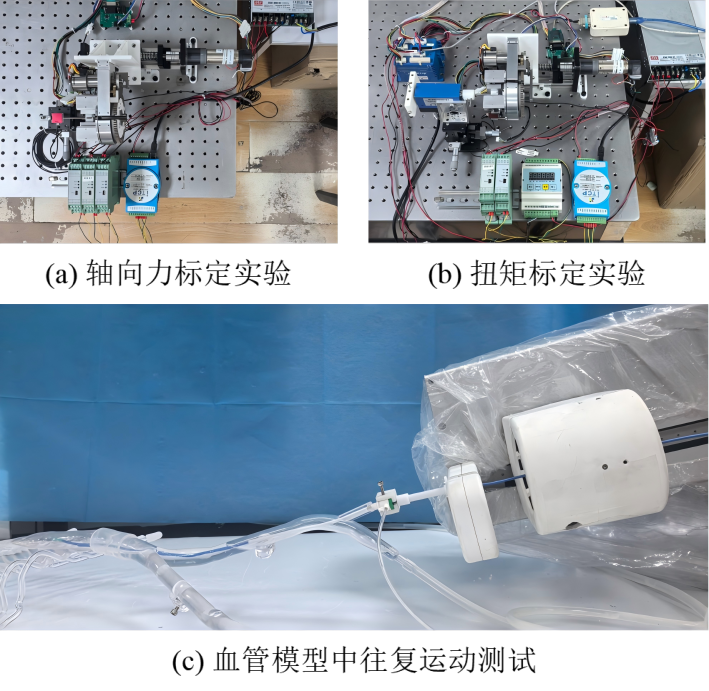
\includegraphics[width=\linewidth]{fig4.png}
\bicaption{测量参数标定与往复递送实验设置}{Experimental configurations for measurement calibration and reciprocating delivery}
\label{fig5}
\par\smallskip{\small [待补图中标注：主、副夹爪，轴向与切向测力支路，标准传感器，远端加载单元及血管模型。]}
\end{figure}
\revend

\revbegin
\subsection{测量参数标定与载荷恢复模型辨识}
\revend

\revbegin
通过静态加载得到 $\bm H_0$ 与 $\ell_s$，通过空载角度扫描得到 $\bm b(\varphi_M)$，通过轴向与旋转启停数据分别辨识 $m_s$ 和 $J_s$。各参数、标定范围和残差统计为[待补]。
\revend

\revbegin
为观察夹爪开合时的承载变化，在交接试次中适当延长S3与S7的保持时间。该组记录中，静止状态下夹爪闭合产生约 $15\sim20\,{\rm ms}$ 的短暂波动，随后无明显轴向载荷转移；S4主爪释放和S8副爪释放分别对应主爪卸载与重新承载。S8末主爪载荷增量占S7末副爪载荷的比例约为 $0.74$。该比例及其测量来源、重复试次统计为[待补]。
\revend

\revbegin
对S9轴向恢复曲线辨识 $\lambda_F$、$\Delta_F$ 和 $D_c$，并由式\eqref{eq:initial-slope}计算初始加载斜率 $k_0$。一组恢复曲线的初始加载斜率约为 $1.28\,{\rm N/mm}$。所观察的典型曲线在约 $3.7\,{\rm mm}$ 处出现峰值，峰后载荷回落约 $0.22\,{\rm N}$；相应曲线、样本范围和统计结果为[待补]。峰值位置及回落幅值随推进速度、停留时间和试验周期的变化另作统计，$D_c$ 的跨周期变化结果为[待补]。
\revend

采用相同的辨识区间分别拟合单指数模型（$\Delta_F=0$）与双指数模型，比较两者对载荷上升、峰值和峰后回落的描述。除整个S9区间的拟合RMSE外，分别报告前 $1\,{\rm mm}$ 和前 $2\,{\rm mm}$ 的拟合RMSE，用于量化部分周期起步段的偏差，结果为[待补]。拟合误差以校正后的实测恢复曲线为基准；反馈误差按式\eqref{eq:reference}的参考载荷计算（3.3节）。

\revbegin
跨周期关系检验包括两部分。首先，将 $\lambda_F$ 对 $\widehat A_{9,F}+\Delta_F$ 作回归，结合各周期 $k_0$ 的分布，检验两者是否近似成正比。其次，对存在有限峰值的周期，按式\eqref{eq:peak-location}计算峰值行程并与实测值比较；单调恢复的周期单独报告其数量。回归系数、拟合区间、峰位误差和对应图表为[待补]。
\revend

$\lambda_F$、$\Delta_F$ 和 $D_c$ 由各速度档数据联合辨识为一组参数。为检查共用一组参数是否合适，另按速度档分别拟合，比较各档参数及其拟合误差与共用参数时的差别。各速度档的参数、拟合误差及差异检验为[待补]。

参考载荷的构造假设用分段恒速连续递送数据检验。在往复递送覆盖的插入深度上，比较S9区间按式\eqref{eq:reference}得到的参考值与相同管路、器械和速度下恒速递送在同一深度的载荷，并以恒速递送同深度重复试验的离散度作为比较基准。若两者差值与重复离散度处于同一量级，则认为S9区间的插值参考可以近似代表不换手递送载荷；差异较大的深度区间在结果中单独标出。深度分段与统计结果为[待补]。

物理参数辨识、网络训练和独立测试按完整试次划分，测试前冻结模型参数及标准化参数。逐周期拟合仅用于分析参数与曲线特征的关系。网络结构取 $M=20$ 个行程单元、$K=10$ 个历史周期、编码维度 $d=32$，第一级为单层单向GRU，第二级为单头注意力，输出为一个轴向残差，可训练参数约 $7.6\times10^3$ 个；$M$、$K$ 与 $d$ 通过验证集选择。训练、验证与测试试次数，优化参数，锁存窗口 $N_{\rm lock}$、行程窗口 $s_{\rm win}$、残差淡入长度 $N_b$、限幅参数 $\eta$ 与 $e_{0,F}$、停止判定参数及撤除时长 $T_{\rm off}$ 为[待补]。

\subsection{对比实验结果与指标分析}

各方法采用同一试次预先确定的阶段边界和评价窗口。轴向力比较以下六种方法。Raw仅作传递矩阵换算，保留原始波动；Kinematic Bias在此基础上扣除惯性和零载基线；ZOH在S2至S9保持S1末锁存值，进入S10后输出校正测量值；Physics Baseline采用轴向恢复模型及本文的阶段切换规则，不加入残差网络；Physics + Coupled GRU在相同补偿流程中，将实时轴向物理基线作为残差网络的附加输入；Physics + Decoupled GRU为本文不含实时测力输入的残差网络。后两种方法采用相同的数据划分、网络规模、限幅和输出过渡设置。扭矩单独评价测量校正与S2～S8锁存的效果，S9直接使用校正测量值。

\subsubsection{参考误差分析}

\revbegin
对稳态递送阶段（S1、S10）和轴向重加载阶段（S9）分别计算均方根误差（RMSE）与平均绝对误差（MAE）。令 $d_p[k]=w_{{\rm fb},p}[k]-w_{{\rm ref},p}[k]$，则
\begin{align}
\label{eq:rmse-mae}
\begin{aligned}
\mathrm{RMSE}_{p,s}&=\sqrt{\frac{1}{|\Omega_s|}\sum_{k\in\Omega_s}d_p^2[k]},\\
\mathrm{MAE}_{p,s}&=\frac{1}{|\Omega_s|}\sum_{k\in\Omega_s}|d_p[k]|.
\end{aligned}
\end{align}
式中，$\Omega_s$ 为相应阶段的样本集合，$p\in\{F,\tau\}$ 为评价通道。交接锁存阶段另行报告误差，不并入稳态递送阶段。在S2～S10的评价窗口内，误差峰峰值定义为
\begin{align}
\label{eq:peak-error}
E_{{\rm peak},p}=
\max_{k\in\Omega_{\rm S2\text{--}S10}}d_p[k]
-\min_{k\in\Omega_{\rm S2\text{--}S10}}d_p[k].
\end{align}
\revend

轴向反馈恢复时间采用绝对误差带定义：
\begin{align}
\label{eq:recovery-time}
\begin{aligned}
t_{\rm rec}={}&\inf\bigl\{t\ge t_{\rm S8,end}:\\
&|d_F(t')|\le\varepsilon_{\rm tol},\quad
\forall t'\in[t,t+t_{\rm win}]\bigr\}\\
&-t_{\rm S8,end}.
\end{aligned}
\end{align}
式中，$t_{\rm win}$ 为连续保持在误差带内的时间，$\varepsilon_{\rm tol}=2\sigma_{{\rm rep},F}$。$\sigma_{{\rm rep},p}$ 由分段恒速递送中同一深度、同一速度的重复试验估计：在各深度计算重复试验间的载荷方差，再取评价深度范围内方差均值的平方根。两通道的重复性分别以力和扭矩单位报告。S1与S10的参考值即校正测量值，该阶段误差主要反映测量校正和阶段切换的影响。观察区间内未满足恢复条件的试次记为未恢复，并列出其数量。误差保持时间与观察区间长度为[待补]。

\revbegin
\begin{table*}[t]
\RevisionColor
\centering
\bicaption{\revised{轴向力反馈的参考误差与恢复表现}}{\revised{Reference errors and recovery performance of axial force feedback}}
\label{tab1}
\small
\setlength{\tabcolsep}{5pt}
\begin{tabular}{p{0.29\textwidth}cccc}
\toprule
对比方法 & \shortstack{S1、S10\\RMSE/MAE (N)} & \shortstack{S9\\RMSE/MAE (N)} & $E_{{\rm peak},F}$ (N) & $t_{\rm rec}$ (s)\\
\midrule
Raw & 待补 & 待补 & 待补 & 待补\\
Kinematic Bias & 待补 & 待补 & 待补 & 待补\\
ZOH & 待补 & 待补 & 待补 & 待补\\
Physics Baseline & 待补 & 待补 & 待补 & 待补\\
Physics + Coupled GRU & 待补 & 待补 & 待补 & 待补\\
Physics + Decoupled GRU & 待补 & 待补 & 待补 & 待补\\
\midrule
参考重复性 $\sigma_{{\rm rep},F}$ (N) & \multicolumn{4}{l}{待补（按工况分别报告）}\\
\bottomrule
\end{tabular}
\end{table*}
\revend

\revbegin
表\ref{tab1}按器械和递送工况汇总轴向结果，各方法的重复试次统计及差异分析为[待补]。扭矩通道报告校正前后的误差、交接锁存期间的输出变化及S9恢复实测输出时的变化，结果与参考重复性 $\sigma_{{\rm rep},\tau}$ 为[待补]。
\revend

\subsubsection{阻力突变响应评估}

在S1稳态递送中途和S9初始恢复阶段，通过远端加载单元施加未参与训练的轴向阶跃阻力，并在相同深度和递送轨迹下设置无扰动的往复递送试次。用有、无扰动反馈波形之差提取阻力增量 $\delta F_{\rm fb}(t)$。参考增量 $\delta F_{\rm ref}(t)$ 取同一加载设定下S1阶跃引起的校正测量增量，S1不受交接影响。阶跃保留比与响应延迟定义为
\begin{align}
\label{eq:step-metrics}
G_{\rm step}&=\frac{\Delta F_{\rm fb}}{\Delta F_{\rm ref}},\\
\Delta t_{63}&=t_{{\rm fb},63\%}-t_{{\rm ref},63\%}.
\end{align}
式中，$\Delta F$ 为增量波形在规定阶跃平台内的均值；$t_{{\rm fb},63\%}$ 与 $t_{{\rm ref},63\%}$ 均从阶跃施加时刻开始计时，分别为反馈增量和参考增量首次达到 $\Delta F_{\rm ref}$ 的63\%所需的时间。未达到该阈值的试次记为未响应。阶跃幅值、施加位置、平台窗口及统计结果为[待补]。重点比较耦合输入与解耦输入残差网络在S9中的幅值保留和响应延迟。

\revbegin
\begin{figure}[H]
\RevisionColor
\centering
\fbox{\parbox{0.92\linewidth}{\raggedright [图6待补：(a) S1稳态递送中的轴向阻力阶跃；(b) S9初始恢复阶段的阶跃响应；(c) 耦合输入与解耦输入残差网络的阶跃保留比和响应延迟。波形标出扰动时刻、参考增量及63\%阈值。]}}
\bicaption{\revised{S1与S9阶段的轴向阻力突变响应}}{\revised{Responses to axial resistance steps during S1 and S9}}
\label{fig6}
\end{figure}
\revend

\subsubsection{消融实验与模型泛化性分析}

以完整方法为基准，分别设置去掉轴向恢复模型、去掉附加衰减项（$\Delta_F=0$）和去掉残差网络的消融变体。各变体采用相同数据划分和评价窗口，含残差网络的变体按各自物理基线重新训练。比较S9误差、前 $1\sim2\,{\rm mm}$ 的误差及全周期波动，结果见图\ref{fig7}。

\revbegin
泛化性评价包括不同推进速度、夹爪预紧力及器械条件。推进速度设置为 $5\,{\rm mm/s}$、$10\,{\rm mm/s}$ 和 $15\,{\rm mm/s}$，预紧力范围和试次分配为[待补]。各测试条件使用冻结参数，分别报告轴向恢复误差和阶跃响应。另记录S9完成、停止和回拉时的补偿撤除波形，以及初始载荷缺口非正时的直接测量输出；参数设置与结果为[待补]。
\revend

\revbegin
\begin{figure}[H]
\RevisionColor
\centering
\fbox{\parbox{0.92\linewidth}{\raggedright [图7待补：(a) 完整方法与三种消融变体的S9轴向误差及全周期波动；(b) 不同速度、预紧力和器械条件下的轴向误差；(c) 完成、停止、回拉及非正初始载荷缺口条件下的输出示例。各图给出重复试次数和统计量。]}}
\bicaption{\revised{轴向补偿方法的消融与不同工况评价}}{\revised{Ablation and operating-condition evaluation of axial compensation}}
\label{fig7}
\end{figure}
\revend

\revbegin
\subsubsection{网络结构与数据量对比}
\revend

网络部分比较四种结构，均使用相同的输入量、训练集、损失函数和评价窗口。单周期变体去掉式\eqref{eq:cross-cycle}的第二级；TCN以因果膨胀卷积替代第一级GRU，卷积核长3、通道32、层数4，在 $M=20$ 个行程单元上的感受野覆盖全部单元；逐点网络不划分行程单元，也不使用前序周期，以逐点输入直接回归残差，隐层宽度按相近参数量选取。四种结构的可训练参数量列于表\ref{tab2}。

\revbegin
为回答训练数据量的问题，取训练试次数 $N_{\rm tr}\in\{10,25,50,100\}$，在相同的验证集上比较四种结构，给出各结构的验证误差随 $N_{\rm tr}$ 的变化。训练集小于全量时按试次抽取，抽取比例固定为10组增量，各结构使用同一组训练试次。另按留一种器械刚度、留一条血管路径分别设置条件留出，报告各结构在未参与训练条件下的误差。训练曲线、拐点位置及各结构的参数量与误差统计为[待补]。
\revend

\revbegin
\begin{table}[H]
\RevisionColor
\centering
\bicaption{\revised{残差网络结构与可训练参数量}}{\revised{Residual network structures and trainable parameters}}
\label{tab2}
\small
\begin{tabular}{lccc}
\toprule
结构 & 周期编码 & 跨周期聚合 & 可训练参数量 \\
\midrule
本文（两级） & 行程单元GRU & 同单元注意力 & 约 $7.6\times10^3$ \\
单周期变体 & 行程单元GRU & 无 & 约 $4.4\times10^3$ \\
TCN & 膨胀卷积 & 无 & 约 $1.1\times10^4$ \\
逐点网络 & 无 & 无 & 约 $7.5\times10^3$ \\
\bottomrule
\end{tabular}
\end{table}
\revend

\revbegin
\subsubsection{血管模型连续递送重构与操作者感知实验}
\revend

\revbegin
在介入血管模型中执行多周期往复推进及伴随旋转的递送任务，记录原始测量、校正测量和反馈输出。轴向波形用于评价换手后的连续力反馈重构，扭矩波形用于观察测量校正、交接锁存及S9直接输出的变化，图\ref{fig8}预留完整记录及局部放大结果。
\revend

\revbegin
操作者实验采用主从递送任务，对比未补偿、传统测量校正和本文轴向连续力反馈三种条件。各条件使用相同的扭矩处理和主端反馈映射，比较因素为轴向反馈方式。由多名操作者沿指定路径递送器械，并完成狭窄或大曲率分叉等高难部位的通过任务。操作者人数、经验分组、熟悉训练、条件执行顺序及每条件重复次数为[待补]。
\revend

\revbegin
介入总时间从任务开始计至器械到达目标位置，通过成功率为成功完成指定高难部位的试次数占该部位总试次数的比例。目标位置、成功判定、失败条件和最长允许时间为[待补]；未完成任务单独报告。按操作者配对汇总各条件的完成时间与成功率，统计方法、结果及差异分析为[待补]。
\revend

\revbegin
\begin{figure}[H]
\RevisionColor
\centering
\fbox{\parbox{0.92\linewidth}{\raggedright [图8待补：(a) 血管模型中多周期轴向力反馈及校正扭矩波形；(b) 交接与S9恢复阶段的局部放大；(c) 不同轴向反馈条件下的介入总时间与高难部位成功率。标明操作者与试次数，扭矩曲线不加入重加载补偿。]}}
\bicaption{\revised{血管模型递送反馈与操作者任务表现}}{\revised{Delivery feedback and operator task performance in a vascular phantom}}
\label{fig8}
\end{figure}
\revend

\section{讨论（Discussion）}

\revbegin
轴向恢复模型将初期载荷增长与随后附加阻力的衰减合并描述。初始加载斜率 $k_0$ 联系了载荷缺口、附加阻力幅值与恢复特征行程；在弹性恢复假设下，较低的加载斜率对应较长的恢复行程。跨周期比例关系及峰位比较结果为[待补]。部分周期起步段与物理模型的偏差由残差网络修正，其贡献通过初始行程误差和消融结果评价。
\revend

残差网络按行程单元组织，而不直接处理逐点序列。一次S9恢复的前向行程为数毫米，所含采样点数随推进速度变化，相邻样本高度相关，逐点序列中的有效样本数远少于采样点数。按行程单元编码后，不同速度下的恢复过程具有相同长度的表示，前序周期的信息也可以按同一行程位置对齐。表\ref{tab2}的结构对比与 $N_{\rm tr}$ 学习曲线用于检验这一设计，结果见3.3.4节。

\revbegin
实测值与补偿量分别进入轴向输出，使恢复模型和残差网络的过渡处理集中于补偿量。阶跃实验评价新增阻力的幅值保留与响应延迟，血管模型实验进一步比较不同轴向反馈条件下的介入总时间及高难部位成功率；相关结果及其对操作者判断受阻状态的影响为[待补]。
\revend

参考载荷由往复递送数据构造，S9区间按插入深度线性插值。这一构造假设不换手时载荷在恢复行程内随深度平缓变化；若该行程内存在局部阻力变化，例如器械尖端进入分支或狭窄段，插值参考会将其平滑，S9的误差评价中将包含这部分偏差。分段恒速连续递送数据用于检验该假设在所测路径上的适用程度。本文结论限于所测的2～3条路径和2种器械刚度，路径或器械改变时需要重新检验。

\revbegin
交接锁存期间（S2～S8）的适用条件为：减速停止后的器械由当前承载夹爪保持，连续递送参考载荷在该短时段内近似不变。扭矩在S9采用校正实测值，长柔器械在弯曲管腔中的扭转储能与甩转未纳入轴向恢复模型。
\revend

\section{结论（Conclusions）}

本文针对往复夹持递送引起的近端测力波动，建立了测量校正、交接受力分析、轴向载荷恢复模型与残差网络修正相结合的反馈方法。以S1末稳态载荷和S8末实测承载确定轴向补偿初值，用前向推进行程描述弹性恢复及附加阻力衰减，并在恢复完成、停止或回拉时平滑撤除补偿。残差网络按恢复行程单元逐单元编码，并对前序周期同一单元的编码进行聚合，不使用实时测力。扭矩通道采用测量校正与交接锁存。参考误差、阶跃响应、结构与数据量对比、消融及操作者实验的定量结论为[待补]。

\noindent
\textbf{数据可用性声明}

\revbegin
[待补：与本研究对应的数据集名称、存储平台、访问链接及开放状态。]
\revend

% -------- 参考文献表
\bibliographystyle{jqr-num}
\bibliography{references}

\begin{AuthorIntroduction}
\Intro 第一作者：隋凯丞（2000--），男，硕士研究生。研究领域：血管介入手术机器人，机器人力感知与控制。E-mail: suikaicheng24@mails.ucas.ac.cn。
\revbegin

\Intro
通信作者：胡琨元（出生年份待补），作者简介与E-mail为[待补]。
\revend

\Intro 通信作者：刘浩（1976--），男，博士，研究员，博士生导师。研究领域：医疗微创手术机器人，智能控制。E-mail: liuhao@sia.cn。

\end{AuthorIntroduction}

\balance
\end{document}
